\addtocontents{xms}{\protect\addvspace{10pt}}
\chapter{Programes d'Aplicació a l'Electrotècnia}\label{chap:python-programes}

\section{Introducció}
\lstset{
	language=Python,
	numbers=left,
	frame=lines,
	morekeywords=[1]{as,None,match,case,with}
}

En aquest capítol es presenten dos mòduls de Python amb funcions útils per resoldre problemes d'electrotècnia; es llisten els  mòduls i es donen petits exemples d'ús. En el capítol \ref{chap:python-exemples} es fan servir aquests dos mòduls per resoldre diversos exemples del llibre.

Per utilitzar aquests mòduls cal crear una carpeta amb el nom \texttt{qed} i copiar-hi els tres fitxers, que es llistaran en les seccions següents: \texttt{\_\_init\_\_.py}, \texttt{utils.py} i \texttt{eng\_elc.py}. D'aquesta manera podrem accedir a les classes i funcions dels mòduls qed.utils i qed.eng\_elc utilitzant la funció \texttt{import} de Python.



\section{Fitxer d'inicialització}
En el llistat \vref{lst:ini} es pot veure el contingut del fitxer d'inicialització  \texttt{\_\_init\_\_.py}.

\lstinputlisting[caption={Python --- Fitxer \_\_init\_\_.py}, label=lst:ini]{Python/qed/\_\_init\_\_.py}

\section{Mòdul d'utilitats}
En el llistat \vref{lst:utils} es pot veure el llistat del fitxer \texttt{utils.py}, el qual conté la implementació del mòdul qed.utils.

\lstinputlisting[caption={Python --- Fitxer utils.py (mòdul qed.utils)},label=lst:utils]{Python/qed/utils.py}

\section{Mòdul de funcions d'enginyeria elèctrica}
En el llistat \vref{lst:eng-elec} es pot veure el llistat del fitxer \texttt{eng\_elec.py}, el qual conté la implementació del mòdul qed.eng\_elec.

\lstinputlisting[caption={Python --- Fitxer eng\_elec.py (mòdul qed.eng\_elec)},label=lst:eng-elec]{Python/qed/eng_elec.py}

\lstset{
	language=Python,
	numbers=none,
	frame=none,
	morekeywords=[1]{as,None,match,case,with}
}

\section{Exemples}
Es donen a continuació  exemples d'ús d'algunes de les funcions d'aquests dos mòduls. S'utilitzen també funcions de les llibreries NumPy i  matplotlib.

\begin{lstlisting}
>>> # Importem primer els mòduls necessaris
>>> import numpy as np
>>> import matplotlib.pyplot as plt
>>> from qed.utils import Complex
>>> import qed.eng_elec as ee
\end{lstlisting} 

\begin{lstlisting}[mathescape=true]
>>> # Comparació de les corbes 51 'very inverse' CEI i IEEE
>>> I_p = 100  # A
>>> I_min = 1.05*I_p  # A
>>> I_max = 5*I_p  # A
>>> I = np.linspace(I_min, I_max, 200)  # A
>>> t_CEI = ee.CEI_51_curve(I, ee.EE.CEI_VERY_INVERSE, I_p)  # s   
>>> t_IEEE = ee.IEEE_51_curve(I, ee.EE.IEEE_VERY_INVERSE, I_p)  # s      
>>> fig, ax = plt.subplots(figsize=(7, 8))
>>> ax.grid(which='minor', alpha=0.2)
>>> ax.grid(which='major', alpha=0.9)
>>> ax.set(yscale="log")
>>> ax.set_ylim(0.1, 1000)
>>> ax.set_xlim(I_p, I_max)
>>> ax.plot(I, t_CEI, label='CEI')
>>> ax.plot(I, t_IEEE, label='IEEE')
>>> ax.set_title("Corbes 51 'very inverse'")
>>> ax.set_ylabel("Temps / s")
>>> ax.set_xlabel("Corrent / A")
>>> ax.legend(loc="best")
>>> plt.show()

$ 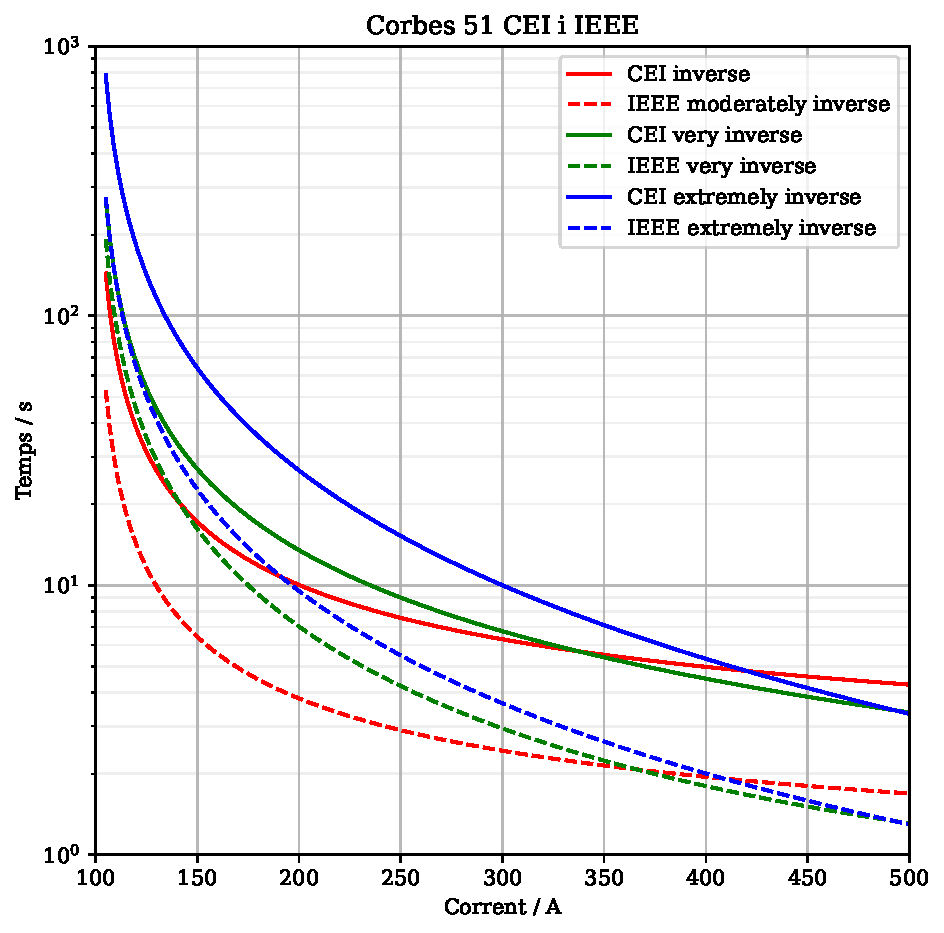
\includegraphics{Cap-PythonProgs-corba51.pdf} $
\end{lstlisting}

\begin{lstlisting}
>>> # Cable trifàsic de 25 mm² de secció i 100 m de longitud
>>> z=ee.z_cable(25, 100)
>>> print(f'Zcable = {z:.4f} Ω/fase = {Complex(z):.4f} Ω/fase')
Zcable = 0.0936+0.0107j Ω/fase = 0.0942∠6.5215° Ω/fase	
\end{lstlisting} 

\begin{lstlisting}
>>> # Cable monofàsic de 25 mm² de secció i 100 m de longitud
>>> z=ee.z_cable(25, 2*100)
>>> print(f'Zcable = {z:.4f} Ω  = {Complex(z):.4f} Ω')
Zcable = 0.1872+0.0214j Ω  = 0.1884∠6.5215° Ω	
\end{lstlisting}

\begin{lstlisting}
>>> # Cable de corrent continu de 25 mm² de secció i 100 m de longitud
>>> z=ee.z_cable(25, 2*100).real
>>> print(f'Zcable = {z:.4f} Ω')
Zcable = 0.1872 Ω	
\end{lstlisting}

\begin{lstlisting}
>>> # Sistema trifàsic: U=380 V fase-fase, I=200 A, cos 𝜑=0.87. Cable: S=240 mm², L=400 m
>>> cdt = ee.voltage_drop(380/np.sqrt(3), 200, ee.z_cable(240, 400), 0.87)
>>> print(f'Caiguda de tensió = {cdt:.2f} V fase-neutre')
Caiguda de tensió = 10.66 V fase-neutre
\end{lstlisting}

\begin{lstlisting}
>>> # Sistema monofàsic: U=220 V, I=55 A, cos 𝜑=0.85. Cable: S=35 mm², L=200 m
>>> cdt = ee.voltage_drop(220, 55, ee.z_cable(35, 2*200), 0.85)
>>> print(f'Caiguda de tensió = {cdt:.2f} V')
Caiguda de tensió = 13.85 V
\end{lstlisting}

\begin{lstlisting}
>>> # Sistema de corrent continu: U=125 V, I=25 A. Cable: S=16 mm², L=50 m
>>> cdt = ee.voltage_drop(125, 25, ee.z_cable(16, 2*50).real)
>>> print(f'Caiguda de tensió = {cdt:.2f} V')
Caiguda de tensió = 3.68 V
\end{lstlisting}

\begin{lstlisting}
>>> # Càlcul d'impedàncies sèrie i paraŀlel
>>> ee.z_series([1+1j, 1+1j, 1+1j])
(3+3j)
>>> ee.z_parallel([3+3j ,3+3j, 3+3j])
(1+1j)
\end{lstlisting}

\begin{lstlisting}
>>> # Resistència unitària d'un fil de 0,5 mm² de secció, a 90 °C 
>>> for material in ["Al", "Cu", "Ag", "Au"]:
. . .   res = ee.r_cable(0.5, 1, 90, material)
. . .   print(f'Material = {material}, Resistència = {res:.4f} Ω/m')
Material = Al, Resistència = 0.0720 Ω/m
Material = Cu, Resistència = 0.0439 Ω/m
Material = Ag, Resistència = 0.0417 Ω/m
Material = Au, Resistència = 0.0604 Ω/m        
\end{lstlisting}

\begin{lstlisting}
>>> # Valors eficaç i mitjà d'una ona senoidal semirectificada
>>> T = 20e-3  # 20 ms
>>> def f(t):
. . .   if t < T/2:
. . .       return 10*np.sin(2*np.pi/T*t)
. . .   else:
. . .       return 0
>>> ee.rms(f, 0, T)  # 10/2
5.0
>>> ee.average(f, 0, T)  # 10/π
3.1830988618379064
\end{lstlisting}

\begin{lstlisting}
>>> # Valors eficaç i mitjà d'una ona senoidal rectificada
>>> T = 20e-3  # 20 ms
>>> def f(t):
. . .   if t < T/2:
. . .       return 10*np.sin(2*np.pi/T*t)
. . .   else:
. . .       return -10*np.sin(2*np.pi/T*t)
>>> ee.rms(f, 0, T)  # 10/√2
7.0710678118654755
>>> ee.average(f, 0, T)  # 2*10/π
6.366197723675812
\end{lstlisting}


